\documentclass[12pt]{report}
\usepackage[english]{babel}
\usepackage{natbib}
\usepackage{url}
\usepackage[utf8x]{inputenc}
\usepackage{amsmath}
\usepackage{graphicx}
\graphicspath{{images/}}
\usepackage{parskip}
\usepackage{fancyhdr}
\usepackage{listings}
\usepackage{csvsimple}
\usepackage{longtable}
\usepackage{vmargin}
\setmarginsrb{3 cm}{2.5 cm}{3 cm}{2.5 cm}{1 cm}{1.5 cm}{1 cm}{1.5 cm}
\usepackage{color}
 
\definecolor{codegreen}{rgb}{0,0.6,0}
\definecolor{codegray}{rgb}{0.5,0.5,0.5}
\definecolor{codepurple}{rgb}{0.58,0,0.82}
\definecolor{backcolour}{rgb}{0.95,0.95,0.92}
 
\lstdefinestyle{mystyle}{
    backgroundcolor=\color{backcolour},   
    commentstyle=\color{codegreen},
    keywordstyle=\color{magenta},
    numberstyle=\tiny\color{codegray},
    stringstyle=\color{codepurple},
    basicstyle=\footnotesize,
    breakatwhitespace=false,         
    breaklines=true,                 
    captionpos=b,                    
    keepspaces=true,                 
    numbers=left,                    
    numbersep=5pt,                  
    showspaces=false,                
    showstringspaces=false,
    showtabs=false,                  
    tabsize=2
}
 
\lstset{style=mystyle}

\title{EY NextWave}								% Title
\author{Marcus Gawronsky}
\date{\today}											% Date

\makeatletter
\let\thetitle\@title
\let\theauthor\@author
\let\thedate\@date
\makeatother

% \pagestyle{fancy}
\setcounter{secnumdepth}{0}

\begin{document}

%%%%%%%%%%%%%%%%%%%%%%%%%%%%%%%%%%%%%%%%%%%%%%%%%%%%%%%%%%%%%%%%%%%%%%%%%%%%%%%%%%%%%%%%%

\begin{titlepage}

   \begin{center}
       \vspace*{5cm}
 
       \textbf{\Huge \thetitle}\\
       \vspace{0.75cm}
        \textbf{\Huge Data Science Competition}
 
       \vspace{1.5cm}
 
       \textbf{\theauthor}

 
       \vspace{0.8cm}
  
       University of Cape Town\\
       South Africa\\
       \today
 
   \end{center}
\end{titlepage}

%%%%%%%%%%%%%%%%%%%%%%%%%%%%%%%%%%%%%%%%%%%%%%%%%%%%%%%%%%%%%%%%%%%%%%%%%%%%%%%%%%%%%%%%%

% \tableofcontents
\pagebreak

%%%%%%%%%%%%%%%%%%%%%%%%%%%%%%%%%%%%%%%%%%%%%%%%%%%%%%%%%%%%%%%%%%%%%%%%%%%%%%%%%%%%%%%%%
\section{Introduction}
This report forms part of an entry in the EY NextWave Data Science Competition 2019.  It outlines the analysis and applications of predictive models trained on a dataset of user GPS data. The report provides details on how to replicate the analysis performed, as well as a criteria for evaluating the chosen model.  
  
\section{Reproducibility}
The analysis in the report was performed using Python 3.7.3 on Ubuntu 19.04. A full list of package dependencies along with the code used to run the analysis is provided in the appendix and can be installed and executed using Anaconda 4.6.11 or using the latest Miniconda Docker Container.  \\
\\
\section{Data}
The datasets provided for the competition came split into a training and test-set with 814262 and 202937 entries respectively. The table below provides a sample of the data containing datapoints trips by individuals.  Each individual is given a \textit{hash}, which is reset each day, and each trip is given a unique \textit{trajectory\_id}.  \\

\begin{center}
\begin{tabular}{ llllllllllll}
\textbf{hash} & \textbf{trajectory\_id}                      & \textbf{time\_entry}                                  & \textbf{time\_exit} & \textbf{vmax}     & \textbf{vmin} & \textbf{vmean}  \\
005... & traj\_005a... & 10:20:00   & 10:28:17 & 0.0  & 0.0   & 0.0 \\
005... & traj\_005a... & 10:40:51   & 10:52:47 & NaN  & NaN   & NaN \\
005... & traj\_005a... & 11:22:09   & 11:45:23 & 0.0  & 0.0   & 0.0
\end{tabular}
\end{center}

\begin{center}
\begin{tabular}{llllllllllll}
    \textbf{x\_entry} & \textbf{y\_entry}     & \textbf{x\_exit}       & \textbf{y\_exit}\\
      3.758e+06 & -1.904e+07 & 3.75e+06 & -1.905e+07\\
      3.759e+06 & -1.911e+07 & 3.75e+06 & -1.913e+07\\
      3.767e+06 & -1.920e+07 & 3.77e+06 & -1.912e+07\\
\end{tabular}
\end{center}

In the table below, one can see imaged which show the distribution of individuals, based on their GPS locations at different points accross the day.  One can see that as the day progresses, we see a greater density of individuals in the city centre.  \\
\begin{center}
\begin{tabular}{|l|l|l|l|l|}
\hline
\textbf{Time} & \textbf{Image}\\
\hline
00:00 & 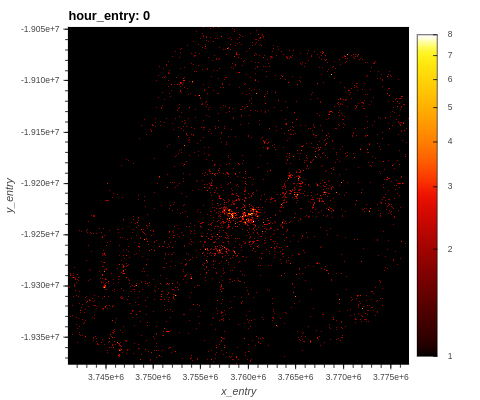
\includegraphics[scale=0.35]{./images/bokeh_plot_(1).png} \\
\hline
05:00 & 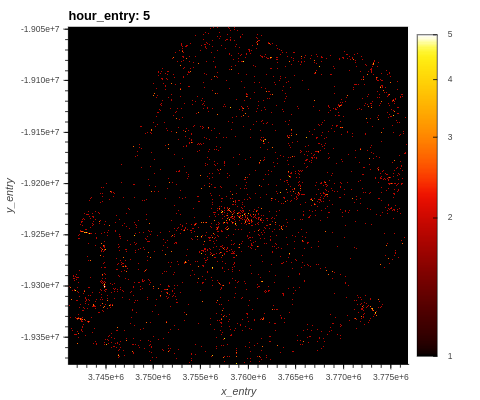
\includegraphics[scale=0.35]{./images/bokeh_plot_(2).png} \\
\hline
10:00 & 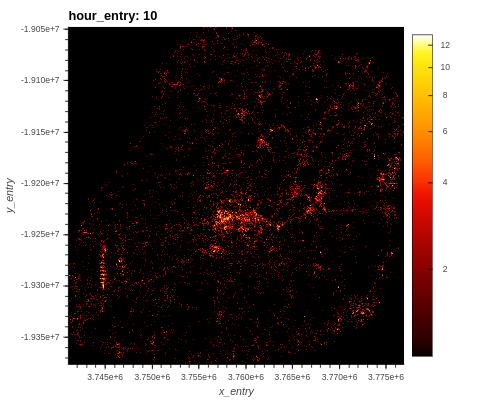
\includegraphics[scale=0.35]{./images/bokeh_plot_(3).png}\\
\hline
15:00 & 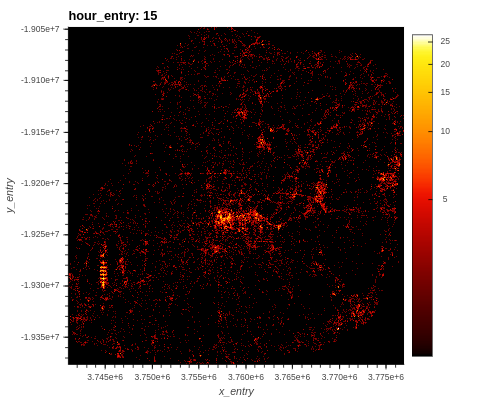
\includegraphics[scale=0.35]{./images/bokeh_plot_(4).png}\\ 
\hline
\end{tabular}
\end{center}

Given this data the aim of the challenge was two-fold: \\
\begin{enumerate}
    \item{To predict the final location of an individual at 15:00}
    \item{To determine a decision-boundary for what constituted the city-centre in order to determine if individuals were in the city centre or not}
\end{enumerate}


\section{Applications}
There exists a large miriad of application for this data and the application of predictive modelling, as shown in the table below.  While these applications have vastly different requirements in terms of accuracy, explainability and security, they can be broadly split into simulation-based application and non-simulation-based applications.  The primary distinction between these two applications is that in simulation-based applications we require a global model, which given a starting point on a map can continuously predict the next location at which the person is observed. Non-simulation-based models may have different requirements and allow for models which only apply to an individual as so do not generalize to arbitary groups of users.  \\
\begin{center}
\begin{tabular}{|l|l|l|}
\hline
\textbf{Simulation}          & \textbf{Non-simulation}                    \\ \hline
Disaster Relief              & \textbf{Fraud detection (Credible credit card use)}\\ \hline
Infectious Disease Modelling & Policing (Testimony, finding suspects)       \\ \hline
Urban Planning               & Marketing/ Product Placement               \\ \hline
\end{tabular}
\end{center}

While the simulation distinction is import, other applications may have different requirements such as explainability or a requirement in quantifying uncertainty.  \\
\newline
Applications such as Fraud detection would use GPS coordinates of an individual given through a cellphone or records of where last a transaction was made in order to try determine if it was likely the person made the next transaction.  In this application, location is not the only priority, security and the quantification of risk or uncertainty is vitally important is we may set a threshold for the the probability of a person being at an store in order to determine if the card has been duplicated.  Similarly we may prefer models which have the ability to be better secured along with the users data and which may be stored and used on edge devices, such as credit card machine or EPOS devices.  

\section{Priorities}
In order to best determine our ideal application and methodology, we must first determine a framework by which to consider and evaluate these use-cases.  These can be broken up into four main subsections: Sustainability, Security, Resources and Predictive Requirements.  

\subsection{Sustainability}  
A major consideration in decising upon our applications is around sustainability. In order to identify if our application is sustainable we need to determine if there a market or need for such as product which can cover even server costs and development. We also need  to determine if certain applications have requirements for greater or continuous data aquisition and whether the market allows for that.  \\
\\
Arguable, all the application present some oppotunity for sustainability and have different markets in which they may compete.  However, while simulation-based methods require little in terms of further data aquisition, our non-simulation-based methods may require continuous data aquisition of where individuals are or have been in order to provide utility.  \\
\\
While this is not a limiting factor applications such as Marketing/ Product Placement may lack the sufficient incentives on the part of users to provide such data in order to optimally  market to them.  In the case of Google Maps, the incentives do work by providing users with a facility by which to navigate and valuable recommendation in exchange for marketing data.  \\

\subsection{Security}
Security is a major consideration for Data Science and IT applications and is a concern which has been growing by legislators and individuals.  In the table below a list of security concerns and examples or explanations is provided:\\ 
\begin{center}
\begin{tabular}{|l|l|}
\hline
\textbf{Type}           & \textbf{Example}                                                                                                                        \\ \hline
Fooled by Data          & 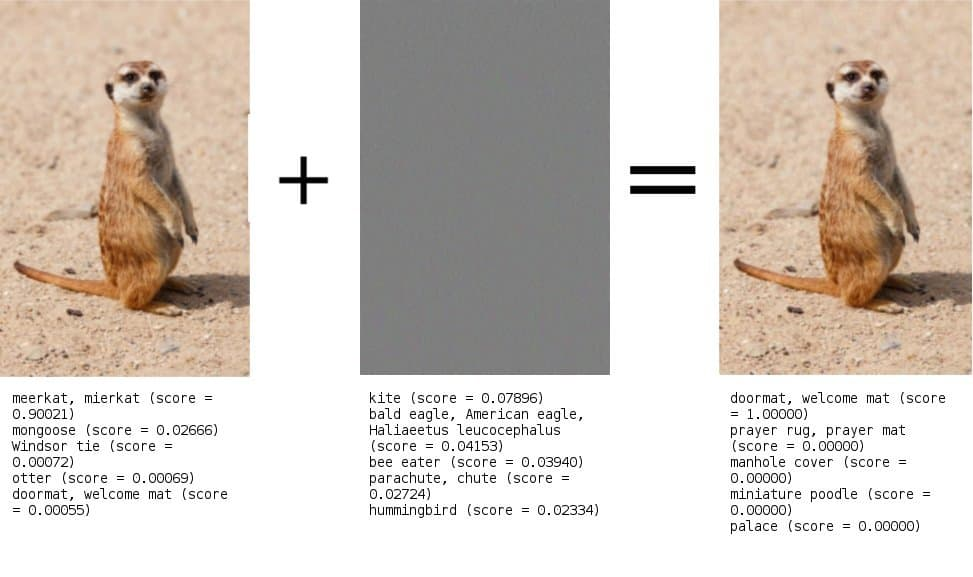
\includegraphics[scale=0.3]{../Media/AdverserialExamples.png}                                                                                                                      \\ \hline
Adverserial Model Drift & Agents feed false data                                                                                                                  \\ \hline
Model Leaks             & 1. Access to accurate global model \\
& \space (GPS spoof me to learn about you) \\
& 2. Parameterizes personal data \\
& \space (Leaks means I know where you live) \\ \hline
Data Leaks              & Centralized data is accessed                                                                                                            \\ \hline
\end{tabular}
\end{center}

A major trade-off in our application is the need for a centralized vs a distributed model.  A centralized model is one in which all individuals are captured by a single model which must be centrally trained and queried by all users.  While such models can scale, they necessitate data being centralized, which creates a risk or security leaks, and provide a tools which malicous agents can use in order to perform queries about the movements of other individuals.  For example, if I have a model which only works for me and which I only have access to then if I put in your location it will not tell me where you will likely be next, however if I have a model which can make predictions about all individuals, I can spoof the model with your coordinates and determine where you will be.  Given the concerns over our the privacy of our data and application this renders simulation-based applications less desireable, as they rely on a centralized model.  \\
\\
Similarly models such as random forests, which paramterize data through decision-rules (such as \textit{if the person is at this location then they will be at this location} given us information about a persons location and) may be less preferable as they raise the security concerns about malacious agents gaining access to either our model or our data, not just the data.  While this concern may be handles in some may through data obfuscation, this still remain a criterea for evaluation.  \\
\\
Lastly, as with many Deep Learning, concerns must be raised in certain applications about our ability to have assurances about our model, as with many cases our inability to properly reason about the model means, as with images, they adding noise to images can lead to castly inaccurate results, which may allow persons to trick models or feed it data which renders it less accurate over time without us knowing or being easily able to identify.  \\

\subsection{Resources}
Across many applications an unavoidable limitation is resource constraints.  Algorithms which rely on matrix factorization do no scale to large datasets easily, as they require all the data being in memory and are thus heabily io-bound.  Similarly extremely Deep Neural Networks can be gigabytes in size and can require specialized and expensive hardware in order to use or may require communication with a server, limiting their application.  

\begin{center}
\begin{tabular}{|l|l|l|l|}
\hline
\textbf{Scenario} & \textbf{Method}         & \textbf{Cheap} & \textbf{Scallable} \\ \hline
Embedded System   & Least-square Regression & Yes            & No                 \\ \hline
Large cluster     & Alex-net (Deep CNN's)   & No             & Yes                \\ \hline
\end{tabular}
\end{center}

\subsection{Predictive Requirements}
Different models and applications have different predictive requirements.  In the table below, we detail three main requirements: Correctness, Confidence and Explainability.  Correctness, here, is the accuracy of a given model which can mean common loss functions like Mean Squared-Error or Binary Cross-entropy, which may be evaluated using some form of validation, such ass using a Test-Train-Split or using Stratified K-fold Cross-validation. \\ 
\\
Confidence asks whether our prediction gives some measure of uncertaintly of its estimate.  For many classification tasts, using Binary cross-entropy a pseudo-probability is specified using a link function and using our loss function a probaility distribution is assumed, meaning we have some assumptions of the distribution of our uncertainty and some quantization in the form of a pseudo-probability. In many bayesian methods the uncertainty of our predicted output can be extensive, in which we are given a probability distribution of an output and can use a range of methods for point estimation based on the risk tolerance of the application.  \\
Lastly, in explainability, some models allow for various levels of explainability in determining what variables in our data and what parameters led to such a prediction.  Here linear models and simple decision tree provide high levels of explainabilitu and assurance, many deep learning methods provide limited methods by which to explain a given prediction.  \\
\begin{center}
\begin{tabular}{|l|l|l|l|}
\hline
\textbf{Example}     & \textbf{Correctness} & \textbf{Confidence} & \textbf{Explainability} \\ \hline
Siri                 & High                 & Low                 & Low                     \\ \hline
Stock Prices         & High                 & High                & Low                     \\ \hline
Macroeconomic Models & Low                  & High                & High                    \\ \hline
Medical Imaging      & High                 & High                & High                    \\ \hline
\end{tabular}
\end{center}

Looking at the table above, applications such as Siri demand the model used in that application to be correct or users become frustrated, but the certainty of a particular prediction or the ability to explain why a particular response was given is not particularly important.  Alternatively in stock prediction, quantifying uncertainty is crucial in deciding optimal asset allocation.  \\
\\
In our applications discussed, applications such as Fraud Detection and Disaster Relief require high levels of correctness and confidence, as we need to know crucially the confidence of a prediction in order to make an optimal decision.  \\


\section{Methodology}
From the framework above, it is clear there are obvious downsides to the large centralized models required for simulation-based application, both in terms of the resources requirements and the security risks.  \\
\\
Given these constraints, we must then tackle the issue of sustainability.  Looking at Fraud Detection, much of the infrastructure is currently in place for businesses with a wide distribution of customer app installs, EPOS devices and credit card machines for data collection.  A clear metric exists to evaluate the value to the business and models can easily be used along with other datasets and models already present in the business.  \\
\\
With this application it is clear that correctness, confidence and security are the primary concerns.  Using Bayesian Modelling we can specify a seperate model unique to each person, which provides us a probability distribution for their location at a point in time.  Here, we can make use of some basis explansion to create polynomial and piecewise functions of time and use Bayesian Ridge Regression, with a differing prior, in order to find an optimal basis in determining the location of a user at a point in time.  \\
\\
For this analysis, rather than looking at the data as a series of entries and exits, we just look at the locations of individuals at points in time, using the following model:  
$$y_{p,i} = \beta_{0,p} + \beta_{1,p} t_{p,i} + \beta_{2,p} t_{p,i}^2 + \beta_{3,p} t_{p,i}^3 + \beta_{4,p} B(||t_{p,i}-\text{10:00am}||_{+})$$  
$$x_{p,i} = \beta_{0,p} + \beta_{1,p} t_{p,i} + \beta_{2,p} t_{p,i}^2 + \beta_{3,p} t_{p,i}^3 + \beta_{4,p} B(||t_{p,i}-\text{10:00am}||_{+})$$  
$$B(t) = x^2 log(x)$$\\
  \\
$p$ is a person with parameter ($\beta$) and times ($t$)\\
$i$ is a point in time ($t$)  \\
$y_{p,i}$, $y_{p,i}$ are the longitude and latitude of an individual\\
$\beta_{k,p}$ are the parameters of each model used for each person\\
\\
In order to fit our model, we used the specification foundin Tipping (2001) and MacKay (1992).  This defines the distribution over our weights of:\\
$$Pr(\beta|\lambda) = N(\beta|0,I\lambda^{-1})$$
The priors for $\lambda$ are chosen to be gamma distributions, using the conjugate prior for the precision of the Gaussian Distribution.  Non-informative priors were chosen for our hyperparamters of $10^{-6}$.  \\

This model was tested over a range of Basis Functions, an example of a predicted path is shown in red below against the path of the user:  \\
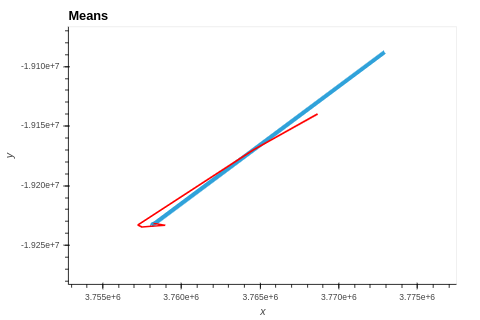
\includegraphics[scale=1]{./images/bokeh_plot_(5).png}

A final decision boundary for the city was chosen to be the 75th and 25th quantiles over our GPS coordinates throughout the day over the longitude and lattitude.  This gave an f1 score of 0.72.  \\

\section{Conclusions}
While model does not provide state of the art accuracy compared to other approached, this approach offers a miriad of advantages in security, scalability, explainability, compute and confidence.  The abilty to analyze a moving probability distribution of the possible location of an individual over time as they move over a map, given their past movements provides a range of advantages, aiding decision-making across a range of applications.  \\

\newpage
\appendix
\section{Appendix}
\subsection{Anaconda Python Dependencies}
\lstinputlisting[]{../environment.yml}
\subsection{Model}
\lstinputlisting[language=Python]{../Model.py}


\section{Bibliography}
Section 3.3 in Christopher M. Bishop: Pattern Recognition and Machine Learning, 2006\\
\\
David J. C. MacKay, Bayesian Interpolation, 1992.\\
\\\
Michael E. Tipping, Sparse Bayesian Learning and the Relevance Vector Machine, 2001.\\

\end{document}